\documentclass[border=.1cm]{standalone}
\usepackage{tikz}

\begin{document}
	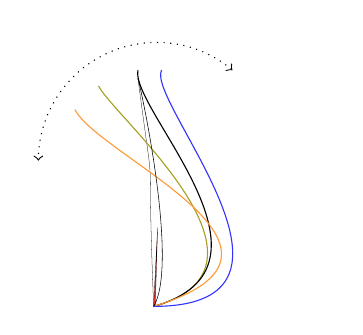
\begin{tikzpicture}	[scale=1]
	
	% antitragus
	\draw[ultra thin] (0,-0.1) .. controls (0.25, -2) and (0.1, -0.5) .. (0.2,-3); % posterior edge
	\draw[thin, olive!80] (-0.5,-0.2) .. controls (-0.3, -0.6) and (2, -2.5) .. (0.2,-3);
	\draw[ultra thin, fill=red!80] (0.2,-3) -- (0.25, -2) -- (0.22, -3); % tragus
	\draw[] (0,0) .. controls (-0.1, -0.5) and (2, -2.5) .. (0.2,-3); % main position
	\draw[thin, orange!80] (-0.8,-0.5) .. controls (-0.5, -1.1) and (2.5, -2.3) .. (0.2,-3);
	
	
	\draw[thin, blue!80] (0.3,0) .. controls (0.1, -0.4) and (2.5, -3) .. (0.2,-3);  
	 
	
	
	\draw[very thin,](0.2,-3) ..controls (0.5, -2.5) and (0.1, -0.5) .. (0,-0.1); % anterior edge
	
	
	\draw[thin, dotted, <->] (1.2,0) arc (50:180:1.5);
	 \useasboundingbox (-1.4,0);
		
	\end{tikzpicture}
\end{document}